\documentclass[a4paper]{report}
\usepackage{graphicx}
\usepackage{array}
\usepackage{natbib}
\usepackage{hyperref}
\usepackage[english]{babel}
\usepackage{lscape}
\usepackage{longtable}

\begin{document}
\begin{titlepage}
\begin{center}
\textsc{\LARGE Contextproject Programming Life}\\
\vspace{5pt}
\textsc{\LARGE Group 2 - GEVATT}\\
\vspace{5pt}
\textsc{\LARGE Final Report}\\
\vspace{5pt}
\textsc{\large TU Delft}

\begin{table}[ht]
\centering
\begin{tabular}{ccc}

\includegraphics[scale=0.2]{ruben.png}   &

\includegraphics[scale=0.2]{mathijs.png} &

\includegraphics[scale=0.2]{jasper.png}  \\
Ruben Bes	& Mathijs Hoogland	& Jasper Denkers\\
rbes 		& mhhoogland 		& jdenkers\\
4227492 	& 4237676 			& 4212584\\
\end{tabular}
\end{table}

\begin{table}[ht]
\centering
\begin{tabular}{cc}
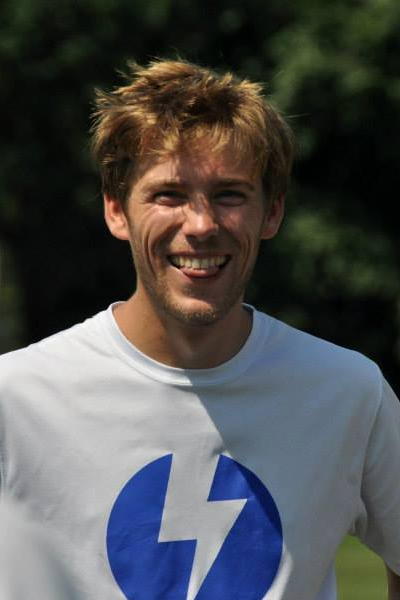
\includegraphics[scale=0.2]{robbert.png} &

\includegraphics[scale=0.2]{willem.png}  \\
Robbert van Staveren	& Willem Jan Glerum\\
rhvanstaveren 			& wglerum\\
1527118					& 4141040\\
\end{tabular}
\end{table}

\vfill
{\large \today}
\end{center}

\end{titlepage}

\begin{landscape}
\setlength\extrarowheight{5pt}
\begin{longtable}{p{6cm}|l|l|l|p{2cm}|p{7cm}}

\textbf{Task} & \textbf{Effort} & \textbf{Assignment} & \textbf{Actual effort} & \textbf{Done} & \textbf{Notes}\\
\hline \hline

Show CADD score in patient overview visualization & 4 & Mathijs & 6 hours & Yes & Was a challenge to distill the right information from a function someone else made. QueryProcessor.java and Mutation.java needed refactoring\\
Show relevant information per chromosome in patient overview visualization & 4 & Mathijs & 1 hour & No & Have not yet found a good way to divide the mutations\\
Sort mutations per column in patient overview visualization & 3 & Mathijs & 4 hours & Yes & Quite easy one the right third-party library was found \\
Show a starting point of a mutation in the mutation view & 3 & Willem Jan & 4 hours & No & Need to find external information first\\
Look if other genes are near the location of a mutation & 3 & Willem Jan & 3 hours & No & Have only made a start, again, external information is needed\\
Implement database testing & 5 & Willem Jan \& Ruben & 7 hours & No & Mostly done by Ruben. Have tried using PowerMock, but had trouble with queries returning a ResultSet. Then tried using PowerMock in combination with MockRunner to make a mocked ResultSet, but due to mismatching types this failed. We have decided to create a test database instead of mocking\\
Make information in the query processor clear (gen vs. protein etc.) & 3 & Ruben & 2 hours & Yes & Changed a few names to match whether a protein or gene was mentioned\\
Add annotations in the mutation view & 3 & Ruben & 2 hours & Yes & None\\
Write query to find all interactions including strengths in a set of proteins & 3 & Ruben & 3 hours & Yes & None\\
Make highlights work in the patient overview page & 3 & Ruben & 3 hours & Yes & Easy once I found out how to use on() in jQuery in combination with hover (or mouseenter and mouseleave in this case) \\
General visualization of protein interaction & 10 & Jasper & 25 hours & Yes & The basics are done, but after our meeting with the client we discovered they wanted the possibility to click on a protein and inspect the interactions of that protein. This will be done the rest of this sprint as well as next week.\\
Visualize protein information per node in the mutation view & 5 & Jasper & 2 hours & No & Have put more time in other visualizations to make them more solid\\
Show strength of relations in the mutation view & 3 & Jasper & 3 hours & Yes & Had to extend the library we use to support different line widths\\
Make a vision about the color usage in the mutation view & 2 & Jasper & 1 hour & No & Have given it some thought, but need to change the query parser to supply the first node\\
Look for a way to save retrieved data & 2 & Robbert \\
Repair the Jenkins server & 2 & Robbert \\
Re-factor parsing protein relation data & 4 & Robbert \\
Extend parser for protein graph (connections with other connections) & 3 & Robbert
\end{longtable}
\end{landscape}

\section*{General Reflection}
After comments we received about not using Git the way it was supposed to be used, e.g. with branches, we decided to make a couple of branches so we could develop in parallel. However, prior to our meeting with the client on Wednesday we merged our branches in order to have the full functionality. These merges broke our application in several places, and Willem Jan spent most of his time fixing these. At the moment, everything has been repaired and we are fully functional again. Besides the merging slowing us down, we (and the other Programming Life group with the same project) had a lot of trouble logging in to STRING, CADD and dbSNP because of too many open connections. It turns out we were somehow causing these, resulting in a whopping 750 open connections, basically making it near impossible to access the databases with our credentials. Again, mainly Willem Jan has been working to fix this. We are still unsure how this happened as we are using try-with-resources, but at least it is back to normal.\\\\
We have also realized this week that the visualizations take more time than expected. This is mostly because we either have to make them ourselves, or need to find libraries which may or may not have to be extended.
\end{document}